% Options for packages loaded elsewhere
\PassOptionsToPackage{unicode}{hyperref}
\PassOptionsToPackage{hyphens}{url}
%
\documentclass[
]{article}
\usepackage{amsmath,amssymb}
\usepackage{iftex}
\ifPDFTeX
  \usepackage[T1]{fontenc}
  \usepackage[utf8]{inputenc}
  \usepackage{textcomp} % provide euro and other symbols
\else % if luatex or xetex
  \usepackage{unicode-math} % this also loads fontspec
  \defaultfontfeatures{Scale=MatchLowercase}
  \defaultfontfeatures[\rmfamily]{Ligatures=TeX,Scale=1}
\fi
\usepackage{lmodern}
\ifPDFTeX\else
  % xetex/luatex font selection
\fi
% Use upquote if available, for straight quotes in verbatim environments
\IfFileExists{upquote.sty}{\usepackage{upquote}}{}
\IfFileExists{microtype.sty}{% use microtype if available
  \usepackage[]{microtype}
  \UseMicrotypeSet[protrusion]{basicmath} % disable protrusion for tt fonts
}{}
\makeatletter
\@ifundefined{KOMAClassName}{% if non-KOMA class
  \IfFileExists{parskip.sty}{%
    \usepackage{parskip}
  }{% else
    \setlength{\parindent}{0pt}
    \setlength{\parskip}{6pt plus 2pt minus 1pt}}
}{% if KOMA class
  \KOMAoptions{parskip=half}}
\makeatother
\usepackage{xcolor}
\usepackage[margin=1in]{geometry}
\usepackage{color}
\usepackage{fancyvrb}
\newcommand{\VerbBar}{|}
\newcommand{\VERB}{\Verb[commandchars=\\\{\}]}
\DefineVerbatimEnvironment{Highlighting}{Verbatim}{commandchars=\\\{\}}
% Add ',fontsize=\small' for more characters per line
\usepackage{framed}
\definecolor{shadecolor}{RGB}{248,248,248}
\newenvironment{Shaded}{\begin{snugshade}}{\end{snugshade}}
\newcommand{\AlertTok}[1]{\textcolor[rgb]{0.94,0.16,0.16}{#1}}
\newcommand{\AnnotationTok}[1]{\textcolor[rgb]{0.56,0.35,0.01}{\textbf{\textit{#1}}}}
\newcommand{\AttributeTok}[1]{\textcolor[rgb]{0.13,0.29,0.53}{#1}}
\newcommand{\BaseNTok}[1]{\textcolor[rgb]{0.00,0.00,0.81}{#1}}
\newcommand{\BuiltInTok}[1]{#1}
\newcommand{\CharTok}[1]{\textcolor[rgb]{0.31,0.60,0.02}{#1}}
\newcommand{\CommentTok}[1]{\textcolor[rgb]{0.56,0.35,0.01}{\textit{#1}}}
\newcommand{\CommentVarTok}[1]{\textcolor[rgb]{0.56,0.35,0.01}{\textbf{\textit{#1}}}}
\newcommand{\ConstantTok}[1]{\textcolor[rgb]{0.56,0.35,0.01}{#1}}
\newcommand{\ControlFlowTok}[1]{\textcolor[rgb]{0.13,0.29,0.53}{\textbf{#1}}}
\newcommand{\DataTypeTok}[1]{\textcolor[rgb]{0.13,0.29,0.53}{#1}}
\newcommand{\DecValTok}[1]{\textcolor[rgb]{0.00,0.00,0.81}{#1}}
\newcommand{\DocumentationTok}[1]{\textcolor[rgb]{0.56,0.35,0.01}{\textbf{\textit{#1}}}}
\newcommand{\ErrorTok}[1]{\textcolor[rgb]{0.64,0.00,0.00}{\textbf{#1}}}
\newcommand{\ExtensionTok}[1]{#1}
\newcommand{\FloatTok}[1]{\textcolor[rgb]{0.00,0.00,0.81}{#1}}
\newcommand{\FunctionTok}[1]{\textcolor[rgb]{0.13,0.29,0.53}{\textbf{#1}}}
\newcommand{\ImportTok}[1]{#1}
\newcommand{\InformationTok}[1]{\textcolor[rgb]{0.56,0.35,0.01}{\textbf{\textit{#1}}}}
\newcommand{\KeywordTok}[1]{\textcolor[rgb]{0.13,0.29,0.53}{\textbf{#1}}}
\newcommand{\NormalTok}[1]{#1}
\newcommand{\OperatorTok}[1]{\textcolor[rgb]{0.81,0.36,0.00}{\textbf{#1}}}
\newcommand{\OtherTok}[1]{\textcolor[rgb]{0.56,0.35,0.01}{#1}}
\newcommand{\PreprocessorTok}[1]{\textcolor[rgb]{0.56,0.35,0.01}{\textit{#1}}}
\newcommand{\RegionMarkerTok}[1]{#1}
\newcommand{\SpecialCharTok}[1]{\textcolor[rgb]{0.81,0.36,0.00}{\textbf{#1}}}
\newcommand{\SpecialStringTok}[1]{\textcolor[rgb]{0.31,0.60,0.02}{#1}}
\newcommand{\StringTok}[1]{\textcolor[rgb]{0.31,0.60,0.02}{#1}}
\newcommand{\VariableTok}[1]{\textcolor[rgb]{0.00,0.00,0.00}{#1}}
\newcommand{\VerbatimStringTok}[1]{\textcolor[rgb]{0.31,0.60,0.02}{#1}}
\newcommand{\WarningTok}[1]{\textcolor[rgb]{0.56,0.35,0.01}{\textbf{\textit{#1}}}}
\usepackage{graphicx}
\makeatletter
\def\maxwidth{\ifdim\Gin@nat@width>\linewidth\linewidth\else\Gin@nat@width\fi}
\def\maxheight{\ifdim\Gin@nat@height>\textheight\textheight\else\Gin@nat@height\fi}
\makeatother
% Scale images if necessary, so that they will not overflow the page
% margins by default, and it is still possible to overwrite the defaults
% using explicit options in \includegraphics[width, height, ...]{}
\setkeys{Gin}{width=\maxwidth,height=\maxheight,keepaspectratio}
% Set default figure placement to htbp
\makeatletter
\def\fps@figure{htbp}
\makeatother
\setlength{\emergencystretch}{3em} % prevent overfull lines
\providecommand{\tightlist}{%
  \setlength{\itemsep}{0pt}\setlength{\parskip}{0pt}}
\setcounter{secnumdepth}{-\maxdimen} % remove section numbering
\ifLuaTeX
  \usepackage{selnolig}  % disable illegal ligatures
\fi
\IfFileExists{bookmark.sty}{\usepackage{bookmark}}{\usepackage{hyperref}}
\IfFileExists{xurl.sty}{\usepackage{xurl}}{} % add URL line breaks if available
\urlstyle{same}
\hypersetup{
  pdftitle={Memo: April 19},
  pdfauthor={Nathan Alexander},
  hidelinks,
  pdfcreator={LaTeX via pandoc}}

\title{Memo: April 19}
\usepackage{etoolbox}
\makeatletter
\providecommand{\subtitle}[1]{% add subtitle to \maketitle
  \apptocmd{\@title}{\par {\large #1 \par}}{}{}
}
\makeatother
\subtitle{Data on Federal and State Prison Population, 1926-1986}
\author{Nathan Alexander}
\date{}

\begin{document}
\maketitle

\hypertarget{title}{%
\section{Title}\label{title}}

\begin{Shaded}
\begin{Highlighting}[]
\CommentTok{\# read in data and update}
\FunctionTok{read\_csv}\NormalTok{(}\StringTok{"/Users/nathanalexander/Dropbox/Projects/prisons/data/fed\_state\_prison\_pop\_1926\_1986.csv"}\NormalTok{,}
         \AttributeTok{col\_types =} \FunctionTok{cols}\NormalTok{(}\AttributeTok{Year =} \FunctionTok{col\_date}\NormalTok{(}\AttributeTok{format =} \StringTok{"\%Y"}\NormalTok{),}
                          \AttributeTok{Total =} \FunctionTok{col\_number}\NormalTok{(),}
                          \StringTok{\textasciigrave{}}\AttributeTok{Total Percentage}\StringTok{\textasciigrave{}} \OtherTok{=} \FunctionTok{col\_number}\NormalTok{(),}
                          \StringTok{\textasciigrave{}}\AttributeTok{Prison Type}\StringTok{\textasciigrave{}} \OtherTok{=} \FunctionTok{col\_factor}\NormalTok{(}\AttributeTok{levels =} \FunctionTok{c}\NormalTok{(}\StringTok{"State + Federal"}\NormalTok{, }\StringTok{"State"}\NormalTok{, }\StringTok{"Federal"}\NormalTok{)), }
                          \StringTok{\textasciigrave{}}\AttributeTok{White Percentage}\StringTok{\textasciigrave{}} \OtherTok{=} \FunctionTok{col\_number}\NormalTok{(),}
                          \StringTok{\textasciigrave{}}\AttributeTok{Black Percentage}\StringTok{\textasciigrave{}} \OtherTok{=} \FunctionTok{col\_number}\NormalTok{())) }\OtherTok{{-}\textgreater{}}\NormalTok{ fed\_state\_prison\_pop\_1926\_1986}
\end{Highlighting}
\end{Shaded}

\begin{verbatim}
## Warning: One or more parsing issues, call `problems()` on your data frame for details,
## e.g.:
##   dat <- vroom(...)
##   problems(dat)
\end{verbatim}

\begin{Shaded}
\begin{Highlighting}[]
\FunctionTok{problems}\NormalTok{(fed\_state\_prison\_pop\_1926\_1986) }\CommentTok{\# identify issues with df}
\end{Highlighting}
\end{Shaded}

\begin{verbatim}
## # A tibble: 4 x 5
##     row   col expected actual file 
##   <int> <int> <chr>    <chr>  <chr>
## 1    25     5 a number -      ""   
## 2    25     6 a number -      ""   
## 3    46     5 a number -      ""   
## 4    46     6 a number -      ""
\end{verbatim}

\begin{Shaded}
\begin{Highlighting}[]
\NormalTok{df }\OtherTok{\textless{}{-}}\NormalTok{ fed\_state\_prison\_pop\_1926\_1986}
\NormalTok{df }\SpecialCharTok{\%\textgreater{}\%} 
  \FunctionTok{rename}\NormalTok{(}\AttributeTok{Count =} \StringTok{\textasciigrave{}}\AttributeTok{Total}\StringTok{\textasciigrave{}}\NormalTok{,}
         \AttributeTok{TotalPct =} \StringTok{\textasciigrave{}}\AttributeTok{Total Percentage}\StringTok{\textasciigrave{}}\NormalTok{,}
         \AttributeTok{Type =} \StringTok{\textasciigrave{}}\AttributeTok{Prison Type}\StringTok{\textasciigrave{}}\NormalTok{,}
         \AttributeTok{WhitePct =} \StringTok{\textasciigrave{}}\AttributeTok{White Percentage}\StringTok{\textasciigrave{}}\NormalTok{,}
         \AttributeTok{BlackPct =} \StringTok{\textasciigrave{}}\AttributeTok{Black Percentage}\StringTok{\textasciigrave{}}\NormalTok{) }\SpecialCharTok{\%\textgreater{}\%} 
  \FunctionTok{relocate}\NormalTok{(Year, Type) }\OtherTok{{-}\textgreater{}}\NormalTok{ df}
\end{Highlighting}
\end{Shaded}

\begin{Shaded}
\begin{Highlighting}[]
\CommentTok{\# subset data}
\NormalTok{df\_state }\OtherTok{=}\NormalTok{ df }\SpecialCharTok{\%\textgreater{}\%} \FunctionTok{filter}\NormalTok{(Type }\SpecialCharTok{==} \StringTok{"State"}\NormalTok{)}
\NormalTok{df\_state}
\end{Highlighting}
\end{Shaded}

\begin{verbatim}
## # A tibble: 41 x 6
##    Year       Type  Count TotalPct WhitePct BlackPct
##    <date>     <fct> <dbl>    <dbl>    <dbl>    <dbl>
##  1 1926-01-01 State 38318      100       75       23
##  2 1927-01-01 State 39041      100       77       22
##  3 1928-01-01 State 42642      100       NA       NA
##  4 1929-01-01 State 49172      100       76       23
##  5 1930-01-01 State 56213      100       75       24
##  6 1931-01-01 State 60905      100       76       23
##  7 1932-01-01 State 57825      100       76       23
##  8 1933-01-01 State 54468      100       74       25
##  9 1934-01-01 State 52976      100       73       26
## 10 1935-01-01 State 53886      100       72       27
## # i 31 more rows
\end{verbatim}

\begin{Shaded}
\begin{Highlighting}[]
\NormalTok{df\_federal }\OtherTok{=}\NormalTok{ df }\SpecialCharTok{\%\textgreater{}\%} \FunctionTok{filter}\NormalTok{(Type }\SpecialCharTok{==} \StringTok{"Federal"}\NormalTok{)}
\NormalTok{df\_federal}
\end{Highlighting}
\end{Shaded}

\begin{verbatim}
## # A tibble: 41 x 6
##    Year       Type    Count TotalPct WhitePct BlackPct
##    <date>     <fct>   <dbl>    <dbl>    <dbl>    <dbl>
##  1 1926-01-01 Federal  5010      100       81       13
##  2 1927-01-01 Federal  5021      100       84       14
##  3 1928-01-01 Federal  5570      100       NA       NA
##  4 1929-01-01 Federal  9734      100       86       12
##  5 1930-01-01 Federal  9800      100       86       12
##  6 1931-01-01 Federal 10615      100       87       11
##  7 1932-01-01 Federal  9652      100       88       10
##  8 1933-01-01 Federal  8333      100       88       10
##  9 1934-01-01 Federal  9275      100       87       11
## 10 1935-01-01 Federal 11837      100       84       14
## # i 31 more rows
\end{verbatim}

\begin{Shaded}
\begin{Highlighting}[]
\NormalTok{df\_both }\OtherTok{=}\NormalTok{ df }\SpecialCharTok{\%\textgreater{}\%} \FunctionTok{filter}\NormalTok{(Type }\SpecialCharTok{==} \StringTok{"State + Federal"}\NormalTok{)}
\NormalTok{df\_both}
\end{Highlighting}
\end{Shaded}

\begin{verbatim}
## # A tibble: 41 x 6
##    Year       Type            Count TotalPct WhitePct BlackPct
##    <date>     <fct>           <dbl>    <dbl>    <dbl>    <dbl>
##  1 1926-01-01 State + Federal 43328      100       78       21
##  2 1927-01-01 State + Federal 44062      100       78       21
##  3 1928-01-01 State + Federal 48212      100       78       21
##  4 1929-01-01 State + Federal 58906      100       78       21
##  5 1930-01-01 State + Federal 66013      100       77       22
##  6 1931-01-01 State + Federal 71520      100       77       22
##  7 1932-01-01 State + Federal 67477      100       77       22
##  8 1933-01-01 State + Federal 62801      100       76       23
##  9 1934-01-01 State + Federal 62251      100       75       24
## 10 1935-01-01 State + Federal 65723      100       74       25
## # i 31 more rows
\end{verbatim}

\begin{Shaded}
\begin{Highlighting}[]
\CommentTok{\# basic plot of state population counts}
\FunctionTok{ggplot}\NormalTok{(df\_state, }\FunctionTok{aes}\NormalTok{(}\AttributeTok{x=}\NormalTok{Year, }\AttributeTok{y=}\NormalTok{Count)) }\SpecialCharTok{+}
  \FunctionTok{geom\_area}\NormalTok{( }\AttributeTok{fill=}\StringTok{"\#69b3a2"}\NormalTok{, }\AttributeTok{alpha=}\FloatTok{0.4}\NormalTok{) }\SpecialCharTok{+}
  \FunctionTok{geom\_line}\NormalTok{(}\AttributeTok{color=}\StringTok{"\#69b3a2"}\NormalTok{, }\AttributeTok{size=}\DecValTok{2}\NormalTok{) }\SpecialCharTok{+}
  \FunctionTok{geom\_point}\NormalTok{(}\AttributeTok{size=}\DecValTok{3}\NormalTok{, }\AttributeTok{color=}\StringTok{"\#69b3a2"}\NormalTok{) }\SpecialCharTok{+}
  \FunctionTok{ggtitle}\NormalTok{(}\StringTok{"US State Prison Counts (1926{-}1986)"}\NormalTok{)}
\end{Highlighting}
\end{Shaded}

\begin{verbatim}
## Warning: Using `size` aesthetic for lines was deprecated in ggplot2 3.4.0.
## i Please use `linewidth` instead.
## This warning is displayed once every 8 hours.
## Call `lifecycle::last_lifecycle_warnings()` to see where this warning was
## generated.
\end{verbatim}

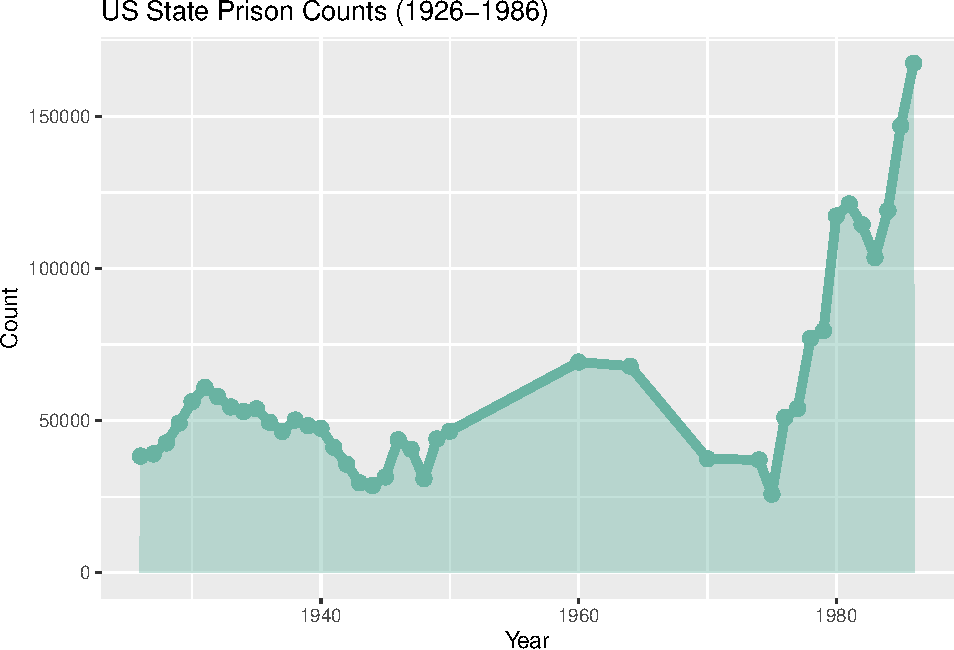
\includegraphics{apr19memo_files/figure-latex/unnamed-chunk-3-1.pdf}

\begin{Shaded}
\begin{Highlighting}[]
\CommentTok{\# basic plot of white vs. black population counts (state + federal)}
\NormalTok{p1 }\OtherTok{\textless{}{-}} \FunctionTok{ggplot}\NormalTok{(df\_both, }\FunctionTok{aes}\NormalTok{(}\AttributeTok{x=}\NormalTok{Year, }\AttributeTok{y=}\NormalTok{WhitePct)) }\SpecialCharTok{+}
  \FunctionTok{geom\_line}\NormalTok{(}\AttributeTok{color=}\StringTok{"lightblue"}\NormalTok{, }\AttributeTok{size=}\DecValTok{2}\NormalTok{) }\SpecialCharTok{+}
  \FunctionTok{ggtitle}\NormalTok{(}\StringTok{"White Percentage"}\NormalTok{)}

\NormalTok{p2 }\OtherTok{\textless{}{-}} \FunctionTok{ggplot}\NormalTok{(df\_both, }\FunctionTok{aes}\NormalTok{(}\AttributeTok{x=}\NormalTok{Year, }\AttributeTok{y=}\NormalTok{BlackPct)) }\SpecialCharTok{+}
  \FunctionTok{geom\_line}\NormalTok{(}\AttributeTok{color=}\StringTok{"darkblue"}\NormalTok{,}\AttributeTok{size=}\DecValTok{2}\NormalTok{) }\SpecialCharTok{+}
  \FunctionTok{ggtitle}\NormalTok{(}\StringTok{"Black Percentage"}\NormalTok{)}
\end{Highlighting}
\end{Shaded}

\begin{Shaded}
\begin{Highlighting}[]
\CommentTok{\# Display both charts side by side thanks to the patchwork package}
\NormalTok{p1 }\SpecialCharTok{+}\NormalTok{ p2}
\end{Highlighting}
\end{Shaded}

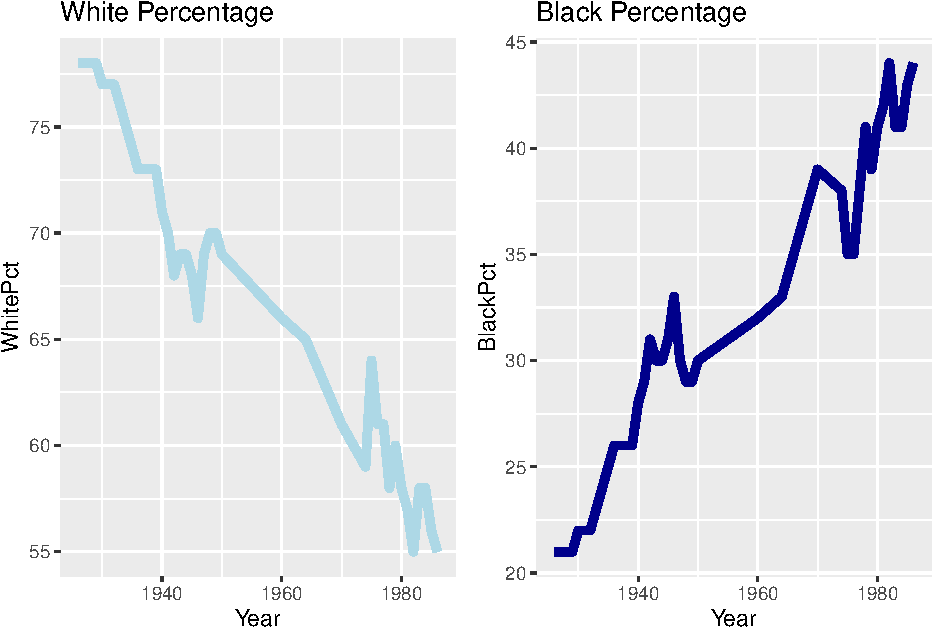
\includegraphics{apr19memo_files/figure-latex/unnamed-chunk-5-1.pdf}

\end{document}
